As we have seen in the preceding chapters there is quite a large range of models designed to generate realistic data such as e.g. images, audio or video. Despite this high diversity only some of them – in particular GANs and VAEs – achieved outstanding success, on the basis of which they were heavily improved in the last years. It is therefore quite difficult to come up with a new model that is able to quickly keep up with these highly adapted models. The fact that in this harsh environment \textit{Score-Based Generative Models} \cite{score_1, score_3, score_2} were able to achieve state-of-the-art results explains why they recently gained a lot of attention and makes them a new promising contender to the field of well established generative models.

\section{The idea behind Score-Based Generative Models}
\sectionmark{The idea behind SGM}
In general the most basic Score-Based Generative Model consists of two core ideas: First, estimating the score $\nabla_{\vec{x}}\log p(\vec{x})$ of an unknown data distribution $p_{data}(\vec{x})$ of a dataset $\{\vec{x}_i\in \mathbb{R}^d\}_{i=1}^N$ of $n$ i.i.d samples. This process is referred to as \textit{Score Matching} \cite{score_matching_original}. And second, using \textit{Langevin Dynamics} \cite{langevin1, langevin2} to sample from the data distribution by staring with an initial value $\tilde{\vec{x}_0}$ from a prior distribution $\pi(\vec{x})$. This value is then gradually transformed by $T$ recursive steps of Langevin Dynamics and will finally come out as $\tilde{\vec{x}}_T$ where $p(\tilde{\vec{x}}_T)\approx p_{data}(\vec{x})$, which makes it a nearly perfect sample of $p_{data}(\vec{x})$. 
%
\subsection{Score Matching} \label{sec:3.1.1}
This section gives an overview of Score Matching and how this technique can be used to get an objective for a score estimator, i.e. the model that is trained to estimate the score $\nabla_{\vec{x}}\log p_{data}(\vec{x})$ of the data distribution $p_{data}(\vec{x})$. The section is mathematically fairly intensive (yet mathematically interesting) and for that reason the main goal of this section is to provide a good feeling for why using the estimation of the score function as a model objective is a reasonable idea.

Score Matching \cite{score_matching_original} is an technique that originates from probabilistic models and their difficulties to be trained on an unnormalized probability density function $\tilde{p}(\vec{x})$ of a data distribution $p_{data}(\vec{x})$. The task of such a model $p_\theta(\vec{x})$ is to learn parameters $\theta$ such that $p_\theta(\vec{x})=p(\vec{x})$ where $p(\vec{x})$ is the normalized density function defined as
%
\begin{equation}
    p(\vec{x})=\frac{\tilde{p}(\vec{x})}{Z},\quad Z=\int\tilde{p}(\vec{x})d\vec{x}\,.
\end{equation}
%
$Z$ is called the partition function and can be understood as a normalization constant. It is this partition function $Z$ that causes the models difficulty to achieve its task. This is because the computation of $Z$ is intractable, meaning that it cannot be solved in polynomial time or rather its complexity is at least $\mathcal{O}(k^n)$. The reason to use the score function to overcome this problem can be easily seen by using some calculation rules for logarithms to get $\log p(\vec{x})=\log\tilde{p}(\vec{x})-\log Z$. It is therefore obvious that the score function $\nabla_{\vec{x}}\log p(\vec{x})$ does not depend on the intractable partition function $Z$.

Score Matching avoids this problematic by minimizing the Fisher divergence between $p_{data}(\vec{x})$ and $p_\theta(\vec{x})$, which is defined as
%
\begin{equation} \label{equ:3.2}
    L(\theta)\triangleq\frac{1}{2}\mathbb{E}_{p_{data}}[\norm{s_\theta(\vec{x})-\nabla_{\vec{x}}\log p_{data}(\vec{x})}^2_2],
\end{equation}
%
where $s_\theta(\vec{x})\triangleq\nabla_{\vec{x}}\log p_\theta(\vec{x})$ and $\norm{\cdot}_2$ is the euclidean norm. From here on we now begin to transition from the probabilistic model $p_\theta(\vec{x})$ to the score model $s_\theta(\vec{x})$. One must understand that in the formulation of Score Matching there is no score model. Score Matching is for probabilistic models. In probabilistic models – to avoid the above mentioned problem with $Z$ – Score Matching is used as a kind of detour. There $s_\theta(\vec{x})$ describes not a model but an score estimator which is then used to further formulate an objective for $p_\theta(\vec{x})$. 

Probabilistic Models aim to learn the data distribution itself. Score-Based Models ($s_\theta(\vec{x})$) aim to learn the score of the data distribution. Therefore no further steps are needed: \cref{equ:3.2} is the objective of Score-Based (Generative) Models. However there are some refining steps left as \cref{equ:3.2} is still not readily usable for leaning score-models because the data distribution $p_{data}(\vec{x})$ is unknown and so is $\nabla_{\vec{x}}\log p_{data}(\vec{x})$. 

%To use \cref{equ:3.2} as an objective it is first transformed to $L(\theta)=J(\theta)+C$ where $C$ is just a constant and $J(\theta)$ is given as
%
%\begin{equation} \label{equ:3.3}
%    J(\theta)\triangleq\mathbb{E}_{p_{data}}\left[\text{tr}(\Delta_{\vec{x}}s_\theta(\vec{x}))+\frac{1}{2}\norm{s_\theta(\vec{x})}^2_2\right].
%\end{equation}
%
%A constant is negligible for a minimization task and the issue with the unknown data distribution has been resolved by introducing the trace $\text{tr}(\cdot)$. The problem with \cref{equ:3.3} is that it is not usable for deep networks and high dimensional data due to the expensive computation of $\text{tr}(\Delta_{\vec{x}}s_\theta(\vec{x}))$. 
To tackle this problem \textit{Denoising Score Matching} \cite{denoise_score} was proposed. Denoising Score Matching introduces noise to \cref{equ:3.2} so that $\nabla_{\vec{x}}$ does not operate directly on the unknown distribution. A noise distribution $q_\sigma(\tilde{\vec{x}}|\vec{x})$ is applied to the data distribution to get a perturbed data distribution $q_\sigma(\vec{x})=\int q_\sigma(\tilde{\vec{x}}|\vec{x})p_{data}(\vec{x})d\vec{x}$. When the noise is small ($q_\sigma(\vec{x})\approx p_{data}(\vec{x})$) then $s_\theta(\vec{x})=\nabla_{\vec{x}}\log q_\sigma(\vec{x})\approx\nabla_{\vec{x}}\log p_{data}(\vec{x})$ holds true. The objective of Denoising Score Matching follows as
%
\begin{equation} \label{equ:3.3}
    \theta^*=\underset{\theta}{\arg\min}\frac{1}{2}\mathbb{E}_{q_\sigma(\tilde{\vec{x}}\lVert\vec{x})p_{data}(\vec{x})}[\norm{s_\theta(\vec{x})-\nabla_{\vec{x}}\log q_\sigma(\vec{x}\lVert\vec{x})}^2_2].
\end{equation}
%
In conclusion \cref{equ:3.3} is the training objective for score based models that is further used throughout this thesis. Nevertheless there are also other Score Matching techniques such as \textit{Sliced Score Matching} \cite{song2019sliced} that could be used but it turns out that Denoising Score Matching is considerably faster. The objective of Score-Based Models (\cref{equ:3.2}) has several desirable properties which makes it a reasonable approach for a generative model. As shown above the objective does not rely on the intractable partition function $Z$. Therefore the objective is almost always tractable which has the implications that there is no special model architecture necessary. Furthermore the objective can be optimized without adversarial training (see GANs) making it easier and more stable to train. %TODO reference GAN section

\subsection{Langevin Dynamics} \label{sec:3.1.2}
As described in \cref{sec:3.1.1} a score-model is tasked to estimate the score of the unknown data distribution $p_{data}(\vec{x})$ of a dataset. However the score of a distribution is not yet a generated image. Instead as it is the \textit{gradient} of the (log) data distribution it can be utilized to sample from $p_{data}(\vec{x})$ by transforming a value $\tilde{\vec{x}}_0$ of a prior distribution $\pi(\vec{x})$ to be part of the data distribution, following the gradient (the score) of the data distribution. There are some restrictions to what the prior distribution should look like but for the considerations of score-based models the prior distribution is just Gaussian noise, so $\pi(\vec{x})\sim\mathcal{N}(\vec{x}, \vec{0}, \vec{I})$.

The process used for sampling is based on \textit{Langevin Dynamics}, a concept from physics, that was adopted to machine learning \cite{langevin1, langevin2}. In Physics the \textit{Langevin Equation} describes particles moving in a potential which additionally are subject to random forces. This process is called Brownian motion. The Langevin equation reads as 
%
\begin{equation} \label{equ:3.4}
    \lambda \frac{\vec{x}(t)}{dt}=-\nabla V(\vec{x}(t))+\vec{\eta}(t),
\end{equation}
%
where $V$ is the potential the particle is moving in, $\vec{x}(t)$ is the particles position and $\vec{\eta}(t)$ is white noise. Commonly \cref{equ:3.4} is written as an (Itô)-Stochastical Differential Equation (SDE)
%
\begin{equation} \label{equ:3.5}
    d\vec{x}(t)=\underbrace{-\nabla V(\vec{x}(t))dt}_\text{drift term}+\underbrace{\sqrt{2}d\vec{w}}_\text{diffusion term}
\end{equation}
%
with a drift term and a diffusion term. $\vec{w}$ denotes the \textit{Wiener Process} which can be interpreted as the derivative of white noise. It is important to note that the positions of particles described by \cref{equ:3.5} are distributed according to some probability density function $p(\vec{x})$ for all times $t\geq0$. This has some very useful consequences: We can choose the potential $V$ in such a way that the underlieing probabilty density function is $p_{data}$. If that is the case we can sample from $p_{data}$.

To achieve the state where the positions particle described by the Langevin Equation are distributed by $p_{data}$ we have to choose $V(\vec{x})=-\log p_{data}({\vec{x}})$. Inserting $V(\vec{x})$ into \cref{equ:3.5} results in
%
\begin{equation} \label{equ:3.6}
    d\vec{x}(t)=\nabla\log p_{data}(\vec{x})dt+\sqrt{2}d\vec{w}.
\end{equation}
%
Now the connection between Sampling with Langevin Dynamics and Score Matching (\cref{sec:3.1.1}) can be seen. If the score of the data distribution is known we can sample from this distribution by using \cref{equ:3.6}. For now $\vec{x}(t)$ was the position of a physical particle but \cref{equ:3.6} is applicable for any $d$-dimensional data $\vec{x}(t)\in\mathbb{R}^d$, e.g. images. To use \cref{equ:3.6} in the context of machine learning a discretized version of the SDE is used:
%
\begin{equation} \label{equ:3.7}
    \tilde{\vec{x}}_t=\tilde{\vec{x}}_{t-1}+\frac{\epsilon}{2}\nabla_{\vec{x}}\log p_{data}(\tilde{\vec{x}}_{t-1})+\sqrt{\epsilon}\vec{z}_t
\end{equation}
%
This equation is a recursive algorithm that can be used to sample from $p_{data}$. Here $\tilde{\vec{x}}_0$ is a value from the prior distribution given above and the $\sim$ above the $\vec{x}$ shows that $\tilde{\vec{x}}$ is not in dataset nor described by the data distribution $p_{data}(\vec{x})$ but a random initial sample. Furthermore $z_t\sim\mathcal{N}(0, I)$ is Gaussian noise and $\epsilon$ is the step size of the algorithm. The sample after $T$ steps is a perfect sample of $p_{data}$ when $T\rightarrow\infty$ and $\epsilon\rightarrow0$. For application of this algorithm $T\gg0$ and $\epsilon\ll1$ are assumed.

Recapitulating what the algorithm does one can look at \cref{fig:3.1}. The lines in the left image show a particle moving randomly according to \cref{equ:3.5}. In the background the underlieing (heartshaped) data density function  is represented and in the right image samples are shown, where each of the dots is an initial sample from the prior distribution that was transformed using \cref{equ:3.7}. When applying \cref{equ:3.7} to infinite values from the prior distribution this process can be thought of as transforming one distribution to another one. As a side-note, the formulation of this integrated process is given by the \textit{Fokker-Planck-Equation} – another important equation in physics. For the purposes of score-based models only a one-by-one application of \cref{equ:3.7} is needed, essentially transforming one image from a noise distribution to an image that looks like it belongs the data distribution of the target dataset.
%
\begin{figure}[] \label{fig:3.1}
    \centering
    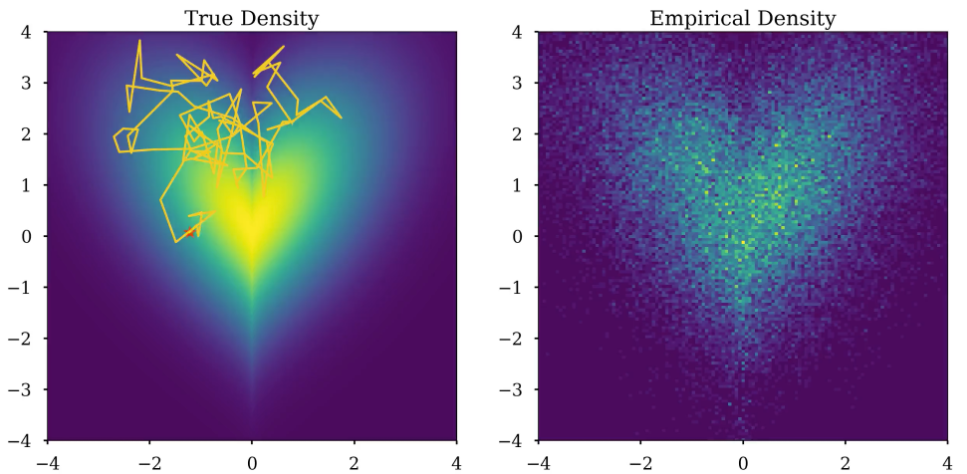
\includegraphics[width=.8\textwidth]{Chapters/figures/langevin.PNG}
    \caption[Short-form caption]{Application of Langevin Dynamics sampling}
\end{figure}
%
\section{Hindrances of a na\"{i}ve applicaton}
While this general concept looks quite appealing to use as a basis for a generative model, in it's na\"{i}ve application it will fail instantly. There are two hindrances preventing this na\"{i}ve application which both are fortunately bypassable by adding random noise to the data. This has also some consequences on Score-Matching and Langevin Dynamics which will be discussed in \cref{sec:3.3}.
%
\subsection{The manifold hypothesis} \label{sec:3.2.1}
The problems in both \cref{sec:3.2.1} and \cref{sec:3.2.2} originate from a similar source: The data density of a dataset of real images. The manifold hypothesis states that real world high-dimensional data lies on low-dimensional manifolds embedded within the high-dimensional space which is called the ambient space. To further explain this hypothesis with an example one can imagine a dataset of black and white images, each image being $m\times n$ in size. The ambient space – the space of \textit{all} possible black and white images with that size – has therefore $m\times n$ dimensions. Datasets normaly do not contain all possible data of a kind which would make them useless but rather contain data that is very special, e.g. images of black and white cars. As there is some similarity in cars the data in such a dataset is assumed to only cover a small, connected volume in the high dimensional space. Mathematically this is called a manifold but it is not important to know this for understanding the hypothesis.

With this hypothesis two problems arise for score-models as they are described above. First, the score $\nabla_{\vec{x}}\log p_{data}(\vec{x})$ is calculated in the whole ambient space, i.e. for all dimensions, not only for the lower dimensions of the manifold. This results in the score being undefined when $\vec{x}$ is confined to such a low dimensional manifold. Second, it was shown in \cite{score_matching_original} that the objective from \cref{equ:3.2} can only be used for defining a consistent score estimator when the data the data distribution describes has the same dimensionality than whole space.
%
\subsection{Low data density region}\label{sec:3.2.2}
A second problem that arises with the data distribution of a dataset of real data is that there is just not enough data to fully cover the data distribution. Recall that the data distribution is unknown and describes \textit{all} data of one kind. To make an example, if a model should learn to generate cars than the data distribution would contain \textit{all} images of cars one can imagine. Certainly we are not able to create a dataset containing images of all cars which in reverse means that the dataset most likely focuses on data that is particularly representative for the data the model should learn.

This has some consequences for score estimation. For data distributions there are regions of high density, where a lot of data is expected. In datasets – as they try to represent the data distribution – most data should appear in this high density regions. But there are also low density regions where little or no data is available. In the car example from above this means that there might be a lot of images of blue or black cars but little or no images of yellow cars. In that regions of low density the score cannot be estimated as there is no data to learn from. In mathematical representation this means that when considering any region $\mathcal{R}\subset\mathbb{R}^d$ in a dataset $\{\vec{x}_i\}_{i=1}^N\overset{i.i.d}{\sim}p_{data}(\vec{x})$ such that $p_{data}(\mathcal{R})\approx0$ the intersection $\{\vec{x}_i\}_{i=1}^N\cap\mathcal{R}$ is often equal to the empty set $\varnothing$. 

\section[Introducing noise to the data distribution]{Introducing noise to the data distribution%
    \sectionmark{Introducing noise}} \label{sec:3.3}
\sectionmark{Introducing noise}
To mitigate the hindrances stated in \cref{sec:3.2.1} and \cref{sec:3.2.2} the data is perturbed with random Gaussian noise. For the problem in \cref{sec:3.2.1} adding small Gaussian noise to the data ensures that the perturbed data distribution has the same dimensionality than the whole space fixing the problem with the inconsistent score estimator. In addition the disturbed data distribution no longer concentrates on a low dimensional manifold so the score is now defined everywhere in ambient space.

The solution to the problem in \cref{sec:3.2.2} is similar but requires large Gaussian noise. This large noise perturbes the data distribution in such a way that low density regions in the original low density region are filled which makes it possible for the score-models to improve on learning the score in low density regions.

The idea is then to use multiple noise levels with decreasing magnitude to transform the maximum noise-perturbed data distribution via a sequence of lower noise-pertubated data distributions to the true (unnoised) data distribution. This idea provokes several changes for the score-model $s_\theta(\vec{x})$ and the Langevin Dynamics sampling procedure.
%
\subsection{Noise Conditional Score Networks}
As there is now a sequence of data distributions with decreasing noise the score-model no longer aims to learn the score of one data distribution but to jointly learn the score of all data distributions. The noise can be thought of as a another parameter besides the data $\vec{x}$. Such a model $s_\theta(\vec{x}, \sigma)$ is called a \textit{Noise Conditional Score Network} (NCSN) \cite{score_1}. In practice when giving the model a value $\vec{x}_\sigma$ from a noisy data distribution $q_{\sigma_i}(\vec{x})\triangleq\int p_{data}(\vec{t})\mathcal{N}(\vec{x}|\vec{t},\sigma_i^2I)d\vec{t}$ the noise $\sigma_i$ of this distribution is given as a second parameter to the model so it can learn the difference between various noise scales applied to data $\vec{x}$. The noise scales $\{\sigma_i\}_{i=1}^L$ are defined as a positive geometric series, i.e. $\frac{\sigma_1}{\sigma_2}=\dots=\frac{\sigma_{L-1}}{\sigma_L}$ where $\sigma_L$ denotes the smallest noise scale and $\sigma_1$ the largest noise scale. If the score-model is properly trained $\forall\sigma\in\{\sigma_i\}_{i=1}^L$ applies $s_\theta(\vec{x}, \sigma)\approx\nabla_{\vec{x}}\log q_\sigma(\vec{x})$.

To achieve high quality samples the model architecture has to be well adapted to the task of noise-conditional Score Matching. As the output of the model is $\in\mathbb{R}^d$ when the input $\vec{x}\in\mathbb{R}^d$ the model architecture of NCSN as described in \cite{score_1} is build upon successful model architectures from dense semantic segmentation a.o. U-Net (\cref{sec:2.1.2}). However, since the implementation of NCSN dramatically changes when advancing to continuous noise scales in \cref{sec:3.4} a more accurate insight to NCSN architecture is first given in \cref{sec:2.4.?}.

In order to train a NCSN the objective of noise-conditional Score Matching must be known. The noise distributions get chosen as $q_\sigma(\tilde{\vec{x}}|\vec{x})=\mathcal{N}(\tilde{\vec{x}}|\vec{x},\sigma^2I)$; therefore $\nabla_{\tilde{\vec{x}}}\log q_\sigma(\tilde{\vec{x}}|\vec{x})=-\nicefrac{(\tilde{\vec{x}}|\vec{x})}{\sigma^2}$. For a given $\sigma\in\{\sigma_i\}_{i=1}^L$ the objective can be formulated as a adaption of \cref{equ:3.3}:
%
\begin{equation} \label{equ:3.8}
    \ell(\theta; \sigma)\triangleq\frac{1}{2}\mathbb{E}_{p_{data}(\vec{x})}\mathbb{E}_{\tilde{\vec{x}}\sim\mathcal{N}(\vec{x},\sigma^2I)}\left[\norm{s_\theta(\tilde{\vec{x}},\sigma)+\frac{\tilde{\vec{x}}-\vec{x}}{\sigma^2}}_2^2\right]
\end{equation}
% 
To get one unified objective \cref{equ:3.8} is summed for all noise scales $\sigma\in\{\sigma_i\}_{i=1}^L$:
%
\begin{equation} \label{equ:3.9}
    \mathcal{L}(\theta;\{\sigma_i\}_{i=1}^L)\triangleq\frac{1}{L}\sum_{i=1}^L\lambda(\sigma_i)\ell(\theta;\sigma_i)
\end{equation}
%
Here $\lambda(\sigma_i)>0$ is a coefficient function depending on $\sigma_i$. As it is advantageous when the scores of all levels of noise have roughly of the same order of magnitude and empirically it is observed that $\norm{s_\theta(\vec{x},\sigma)}_2\propto\nicefrac{1}{\sigma}$, $\lambda(\sigma)$ is chosen to be $\sigma^2$. With that choice the term $\lambda(\sigma_i)\ell(\theta;\sigma_i)$ in \cref{equ:3.9} is equal to $\sigma^2\ell(\theta;\sigma_i)=\frac{1}{2}\mathbb{E}[\norm{\sigma s_\theta(\tilde{\vec{x}},\sigma)+\frac{\tilde{\vec{x}}-\vec{x}}{\sigma^2}}_2^2]$. Because $\frac{\tilde{\vec{x}}-\vec{x}}{\sigma^2}\sim\mathcal{N}(0, I)$ and $\norm{\sigma s_\theta(\tilde{\vec{x}},\sigma)}\propto1$ it is easy to deduce that the order of magnitude of $\lambda(\sigma)\ell(\theta;\sigma)$ is independent of $\sigma$.
%
\subsection{Annealed Langevin Dynamics}
After introducing noice scales is is clear that also the Langevin Dynamics algorithm has to be adjusted. In \cref{sec:3.1.2} we saw that Langevin Dynamics transforms a sample $\tilde{\vec{x}}_0$ from a prior distribution $\pi(\vec{x})$ to a sample $\tilde{\vec{x}}_T$ from the target data distribution $p_{data}$ by applying $T$ steps of Langevin Dynamics algorithm (\cref{equ:3.7}). Now the goal remains the same but it is not possible to directly transform from the prior distribution to the data distribution because the score-model only knows the scores for certain noise levels. Instead \cref{equ:3.7} is applied $L$ times in a sequence, once for each noise distribution $q_\sigma(\vec{x})$. This means that starting from an initial sample $\tilde{\vec{x}}_0$ from a prior distribution that is perturbed with the maximum noise $\sigma_1$ – i.e. $\pi(\vec{x})\sim q_{\sigma_1}(\vec{x})$ – this sample is then transformed to be a sample of the noise distribution $q_{\sigma_{2}}(\vec{x})$. The procedure is then repeated by using the final sample $\tilde{\vec{x}}_T$ from the last step as the new initial sample $\tilde{\vec{x}}_0$ that is then be transformed to be a sample of the noise distribution $q_{\sigma_{3}}(\vec{x})$. After $L$ of such steps we therefore have a sample of $q_{\sigma_L}(\vec{x})\approx p_{data}(\vec{x})$. The final algorithm can be seen in \hyperref[alg:1]{Alg. 1}.
%
\begin{algorithm} \label{alg:1}
    \DontPrintSemicolon
    \Require{$\{\sigma_i\}_{i=1}^L,\epsilon,T$}
    Initialize $\tilde{\vec{x}}_0$\;
    \For{$i\leftarrow$ to $L$}{
        $\alpha_i\leftarrow\epsilon\cdot\sigma_i^2/\sigma_L^2$ \Comment*[r]{$\alpha_i$ is the step size}
        \For{$t\leftarrow1$ to $T$}{
            Draw $z_t\sim\mathcal{N}(0,I)$\;
            $\tilde{\vec{x}}_t\leftarrow\tilde{\vec{x}}_{t-1}+\frac{\alpha_i}{2}s_\theta(\tilde{\vec{x}}_{t-1},\sigma_i)+\sqrt{\alpha_i}\vec{z}_t$
        }
        $\tilde{\vec{x}}_0\leftarrow\tilde{\vec{x}}_T$
    }
    \Return{$\tilde{\vec{x}}_T$}
    \caption{\textsc{Annealed Langevin Dynamics}}
\end{algorithm}
%
Here $\alpha_i$ denotes the outer step size that is tuned down gradually by $\alpha_i=\epsilon\cdot\sigma_i^2/\sigma_L^2$. Since the noise distributions $\{\sigma_i\}_{i=1}^L$ are perturbed with Gaussian noise the scores encountered during sampling are all well defined. Also when $\sigma_1$ is sufficiently large there are less low density regions in $q_{\sigma_1}(\vec{x})$ preventing the algorithm to encounter regions where the score has not been learned due to a lack of training data.

With the release of \cite{score_1} the authors found that their \textit{FID (Fréchet inception distance)} \cite{fid} scores – a metric for evaluating the quality of samples – was lower than state-of-the-art FID scores even though the samples looked better to human eyes. Thereupon \cite{score_4} found that the final sample generated by \hyperref[alg:1]{Alg. 1} contains some noise which is not visible to the human eye but noticeably decreases the FID score. To solve this problem they proposed to add an extra denoising step after the original Annealed Langevin Dynamics which significantly improves FID scores. This improved algorithm can be found in \hyperref[alg:2]{Alg. 2}.
%
\begin{algorithm} \label{alg:2}
    \DontPrintSemicolon
    \Require{$\{\sigma_i\}_{i=1}^L,\epsilon,T$}
    Initialize $\tilde{\vec{x}}_0$\;
    \For{$i\leftarrow$ to $L$}{
        $\alpha_i\leftarrow\epsilon\cdot\sigma_i^2/\sigma_L^2$\;
        \For{$t\leftarrow1$ to $T$}{
            Draw $z_t\sim\mathcal{N}(0,I)$\;
            $\tilde{\vec{x}}_t\leftarrow\tilde{\vec{x}}_{t-1}+\frac{\alpha_i}{2}s_\theta(\tilde{\vec{x}}_{t-1},\sigma_i)+\sqrt{\alpha_i}\vec{z}_t$
        }
        $\tilde{\vec{x}}_0\leftarrow\tilde{\vec{x}}_T$
    }
    \If{denoise $\tilde{\vec{x}_T}$}{
        \Return{$\tilde{\vec{x}}_T +\sigma^2_Ls_\theta(\tilde{\vec{x}}_T,\sigma_L)$}
    }
    \Else{
        \Return{$\tilde{\vec{x}}_T$}
    }
    
    \caption{\textsc{Improved Annealed Langevin Dynamics}}
\end{algorithm}
\section[The way to continuous realms]{The way to continuous realms%
    \sectionmark{Continuous Noise}} \label{sec:3.3}
\sectionmark{Continuous Noise}

\section{Improvements and Adaptations}
\subsection{Mixed precision learning} %0.5-1
vRAM usage and training speed are key aspects in training deep neural network. Complex models might consist of several million up to billion parameters to optimize. This requires an immense amount of computing power but at least equally important, vRAM. vRAM – videa random access memory – is the memory that a GPU has available during operation. Modern high end consumer graphic cards typically have around $10GB$ of vRam. The crux of the matter is that reaching more than $10GB$ when training a moderatly complex model is really easy and when training such complex models as NCSNs, the vRAM demand can increase beyond $100GB$ making training deep neural networks a very cost intensive business. Also when training complex models one can expect to need one week or more of training time making testing and finetuning of models very exhausting.

To mitigate these problems the concept of \textit{Mixed Precision Learning} \cite{mixed_prec} was developed, decreasing both vRAM usage and training time with simultaneous retention of training quality, i.e. training loss. Normally each parameter of a network is stored as a float with $32bits$ of precision. Considering a network with $\sim250M$ parameters this would be equivalent to $\sim1GB$. What sounds not so much at first quickly becomes unmanageable when thinking of the series of matrix arithmetic's the parameters undergo and each calculation storing extra data such as gradients. 

The idea of mixed precision learning is to use floats with a $16bit$ precision wherever possible. In order to not loose model accuracy two concepts are applied. First, there is always a $32bit$ master copy of the model weights. For the forward pass this master copy is converted to $16bit$ where the complex gradient calculations happen. In the backward pass these $16bit$ gradients are converted back to $32bit$ where they are then used by the optimizer to update the master weights. But this improvement during gradient calculation comes with the flaw of loosing some gradients as every number $<2^{-24}$ is equal to $0$ for $16bit$ precision but in most models there is at least some relevant gradient information in the range $[2^{-27},2^{-24})$. To mitigate this effect the concept of loss scaling was proposed. Loss scaling multiplies the $32bit$ loss after the forward pass by a scale factor to move them in the $16bit$ range in which the gradients are then computed in the backward pass. Thereafter the scaled $16bit$ gradients are converted to scaled $32bit$ gradients and then divided by the same scale factor as before. Finally these scaled gradients are used by the optimizer to update the master weights. The full concept can be seen in \hyperref[fig:3.2]{Fig. 3.2}.
%
\begin{figure}[] \label{fig:3.2}
    \centering
    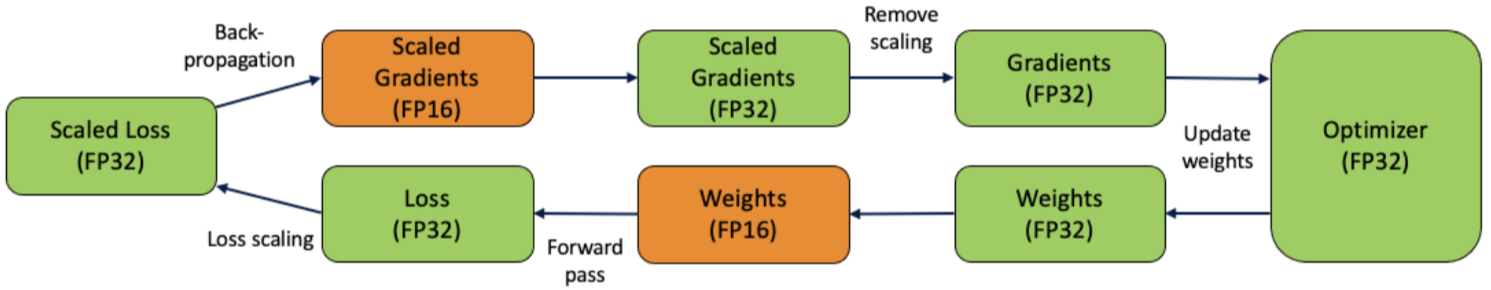
\includegraphics[width=.9\textwidth]{Chapters/figures/mixed_prec.PNG}
    \caption[Short-form caption]{Concept of Mixed Precision}
\end{figure}
%

As the mixed precision technique was not used in the original SGM paper \cite{score_3} it was now implemented using the off the shelf pyTorch tools for mixed precision to check how much this technique improves vRAM usage and training time for the NCSN. To do so the NCSN was trained on the Cityscapes dataset on two different GPUs with the same model settings. For each GPU $2\times100$ epochs were passed, once with mixed precision on and once with mixed precision off. The first GPU was a \textit{Nvidia GeForce RTX 2080 Ti} with $11GB$ of vRAM and the second GPU was a \textit{Nvidia A100} with $40GB$ of vRAM. For both GPUs we used the maximum possible batch size for non mixed precision training which is $1$ for the RTX 2080 Ti and $5$ for the A100. The effects of mixed precision training on vRAM usage and training time can be seen in \hyperref[tab:3.1]{Tab. 3.1} resp. \hyperref[tab:3.1]{Tab. 3.2}. For the vRAM usage the total vRAM needed is shown and for the training time the average training time for one epoch is shown.
%
\begin{table}[] \label{tab:3.1}
        \centering
    \begin{tabular}{c|c|c}
        GPU type        & Mixed precision \textbf{Off}    & Mixed precision \textbf{On} \\
        \hline
        RTX 2080 Ti     &  7791MB               & 7367MB\\
        A100            &  39039MB              & 29481MB
    \end{tabular}
    \caption{vRAM usage w/ and w/o mixed precision}
\end{table}
\begin{table}[b] \label{tab:3.2}
        \centering
    \begin{tabular}{c|c|c}
        GPU type        & Mixed precision \textbf{Off}    & Mixed precision \textbf{On} \\
        \hline
        RTX 2080 Ti     &  1494s                & 1206s    \\
        A100            &  965s                 & 987s
    \end{tabular}
    \caption{Training time per epoch w/ and w/o mixed precision}
\end{table}

For the A100 serious improvements on vRAM usage can be observed. For the RTX 2080 Ti there are only little improvements for vRAM usage but good improvements on training time. In general mixed precision is expected to perform way better on the new Ampere GPU
architecture (A100) than on the older Turing GPU architecture (RTX 2080 Ti). To ensure that the training quality does not suffer from the use of mixed precision the loss curves for all test setups are compared in ... It can be seen that there is no notable effect on training loss. Also a qualitative comparison of generated samples shows no difference perceptible by a human. We therefore conclude that – at least for non FID record breaking attempts – the mixed precision should be used and we do so for all upcoming experiment.

\subsection{Training on arbitrary image sizes} %0.5-1

